\documentclass[journal,10pt,twocolumn]{IEEEtran}
% \documentclass[a4paper, onecolumn, 12pt, doublespacing]{IEEEtran}

\usepackage[noadjust]{cite}
\usepackage{epsfig}
\usepackage{amsmath}
\usepackage{amssymb}
\usepackage{color}
\usepackage{comment}
\usepackage{float}
\usepackage{subcaption}
\usepackage{tikz}
\usetikzlibrary{calc,trees,positioning,arrows,chains,shapes.geometric,%
decorations.pathreplacing,decorations.pathmorphing,shapes,%
matrix,shapes.symbols}

\input{Symbol_Shortcut.tex} % Symbols defined by Victor


\newtheorem{theorem}{\bf Theorem}		% by Victor
\newtheorem{corollary}{\bf Corollary}	% by Victor
\newtheorem{definition}{\bf Definition}	% by Victor

\pagenumbering{arabic}
% \pagestyle{empty}

\makeatletter
\def\ifundefined{\@ifundefined}
\makeatother

\setlength{\parskip}{0ex}

\begin{document}

    %\setlength{\baselineskip}{1.18em}
    %\addtolength{\baselineskip}{-0.1ex}
    %\setlength{\baselineskip}{0.95\baselineskip}


    \title{ Convex Optimization Project Report -\\
    \huge  MMSE Based MIMO Channel Estimator Via Primal-Dual
    Optimization Mehthod with Neural Network}
    \author{312510199 Jing-Hao, Li and 312510197 Zhao-Jie, Luo\\
        Advisor: Professor Carrson C. Fung\\
        \small{Jun. 12, 2024}}
    %\author{Carrson C. Fung$^1$, Man-Wai Kwan$^1$ and Chi-Wah Kok$^2$ \\
    %\small{$^1$Hong Kong App. Sci. \& Tech. Inst., Hong Kong Sci. Park, Shatin,
    %$^2$Dept. of EEE, 
    %Hong Kong Univ. of Sci. \&  Tech., 
    %HONG KONG\\
    %e-mail: \emph{c.fung@ieee.org, mwkwan@ieee.org, eekok@ieee.org}} 
    %\thanks{This work described in this paper has been supported by the Research Grants Council of Hong Kong, China (Project no. CERG HKUST6236/01E)}
    %}

    \markboth{OPTIMIZATION THEORY AND APPLICATIONS}{}

    \maketitle
    % here's how you get a publisher's ID mark with the new
    % IEEEtran.cls.  If you want to use it, don't forget to
    % also uncomment the \pubidadjcol command (which must be
    % executed in the second text column) around line 434 below
    %\pubid{0000--0000/00\$00.00~\copyright~2001 IEEE}

    %\thispagestyle{empty}

    % \begin{comment}
    %     2021 Spring W8 (4/12~4/18)
    %     Coverage: Orthogonality
    % \end{comment}



    % \noindent \textbf{Introduction}
    \section{Introduction}
        
        %%% MIMO part is not needed

        Channel estimation plays a crucial role in communication systems. Its main purpose is to determine the paths through which signals propagate from the transmitter 
        to the receiver and to understand the signal attenuation and distortion along these paths. The accuracy of channel estimation directly impacts the quality of 
        signal decoding at the receiver, making it an essential step in many communication systems.

        In many cases, communication signals are affected by factors such as noise, multipath effects, and interference during transmission, all of which can lead to 
        signal attenuation and distortion. By performing channel estimation, we can better understand these effects and take appropriate compensation measures to ensure 
        the reliable transmission of signals. Channel estimation can also be used to optimize signal transmission and reception strategies, thereby improving system 
        performance and efficiency. 

        In this work, a neural network based minimun mean square estimator, trained using deep reinforcement learning(DRL) and primal-dual optimization technique
        is proposed for MIMO channel estimation. It's posited that the proped estimation will outperform the least-square(LS) and linear MMSE(LMMSE) estimator.

    % \noindent \textbf{Problem setup}
    \section{Problem setup}
    
        Assume that the communication signals are affected by additive white Gaussian noise, fading effects, and phase shift during transmission, consequently,
        the system model can be represented as:
        \begin{equation} \label{eq:sysModel}
            \Y = \H\X + \W,
        \end{equation}

        where $\X \in \mathbb{C}^{n_T \times T}$ represents the transmitted pilot signal, $\W \in \mathbb{C}^{n_R \times T}$ represents the additive white Gaussian noise
        with zero mean and unit variance, $\Y \in \mathbb{C}^{n_R \times T}$ represents the received signal, and $\H \in \mathbb{C}^{n_R \times n_T}$ 
        is the channel matrix containing channel coefficients which represents $n_R \times n_T$ flat fading channel.
        that we aim to estimate. Here, $n_T$ and $n_R$ denote the number of transmit and recieve antennas, respectively. $T$ denotes the multiple of $n_T$, 
        and one unit of $n_T$ is commonly used. Since the column of $\X$ are usually orthonormal, without loss of generality, they are assumed to equal to columns 
        of $\I_{n_T}$.

        Vectorizing (\ref{eq:sysModel}), it becomes 
        \begin{align} \label{vecSysModel}
            \y &= (\X \otimes \I_{n_R})\h + \w \notag \\ &= \tilde{\X}\h + \w,
        \end{align}
        where $\tilde{\X} \triangleq (\X \otimes \I_{n_R}) \in \mathbb{C}^{n_T n_R \times T n_R}.$

    \section{Problem Formulation}

        The MMSE channel estimator aims to minimize the Bayesian MSE of the channel estimate $\hat{\h}$ 
        \begin{equation} \label{eq:mmse1}
            \hat{\h} = \argmin_{\hat{\h}} \mathrm{BMSE}(\hat{\h}),
        \end{equation}
        where
        \begin{equation} \label{eq:bmse}
            \mathrm{BMSE}(\hat{\h}) = \mathbb{E}_{\y,\h}\left[\left\| \h-\hat{\h} \right\|^2_2\right].
        \end{equation}
        The closed-form solution of this MMSE problem is $\hat{\h} = \mathbb{E}_{\h|\y}\left[\h|\y\right]$. However, it requires knowledge about the conditional probability
        $p(\h|\y)$, which may be unknown and/or difficult to obtain. Then (\ref{eq:mmse1}) can be written as
        \begin{equation} \label{eq:mmse2}
            \min_{\hat{\h}} \mathbb{E}_{\y,\h}\left[\left\| \h-\hat{\h} \right\|^2_2\right].
        \end{equation}\\

    \section{Proposed Approach}
    \subsection{Primal-Dual Method}
        (\ref{eq:mmse2}) can be reformulated to its epigraph form as
        \begin{equation}
        \begin{aligned} \label{eq:epi}
            \min_{t,\hat{\mathbf{h}}} \quad & t \\
            \text{s.t.} \quad & \mathbb{E}_{\mathbf{y},\mathbf{h}}\left[\left\| \mathbf{h}-\hat{\mathbf{h}} \right\|^2_2\right] \leq t.
        \end{aligned}
        \end{equation}
        Then its Lagrangian function can be written as
        \begin{equation} \label{eq:Lag1}
            \mathcal{L} \left(\hat{\h},t,\lambda\right) = t + \lambda\left(\mathbb{E}_{\y,\h}\left[\left\| \h-\hat{\h} \right\|^2_2 \right] -t \right)\\
        \end{equation}
        In the MMSE estimator, $\hat{\h}$ is a nonlinear function of y, but its exact form is unknown. Also, since $\h \in \mathcal{H} $, 
        and in turn $\hat{\h} \in \mathcal{H} $, where $\mathcal{H}$ can be interpreted as a set that contains samples of $\h$ (and $\hat{\h}$) from certain 
        unknown distribution or certain (unknown/complicated) channel models. Herein, a neural network (or graph convolution neural network) may be used to
        parameterize $\hat{\h}$ so that $\hat{\h}=\phi(\h;\boldsymbol{\theta})$, with $\boldsymbol{\theta}$ denoting the parameters of the neural network.
        Then the Lagrangian function can also be written as
        \begin{equation} \label{eq:Lag2}
            \mathcal{L} \left(\hat{\h},t,\lambda\right) = t + \lambda\left(\mathbb{E}_{\y,\h}\left[\left\| \h-\phi(\mathbf{y};\boldsymbol{\theta}) \right\|^2_2 \right] -t \right).\\
        \end{equation}
        The dual function can then be written as
        \begin{equation} \label{eq:dual}
            g(\lambda) = \min_{t,\boldsymbol{\theta}}~ t + \lambda\left(\mathbb{E}_{\y,\h}\left[\left\| \h-\phi(\mathbf{y};\boldsymbol{\theta}) \right\|^2_2 \right] -t \right).\\
        \end{equation}
        It is uncertain whether or not the duality gap equals zero.\\
        However, the stationary point of $  \mathcal{L} \left(\hat{\h},t,\lambda\right)$ can be found via the KKT conditions by solving for the primal and dual
        variables alternately using gradient descent and ascent, respectively.\\
        % First, according to the stationarity property of KKT conditions:
        % $\nabla f_0(\x^*) + \sum\limits_{i=1}^{m}\lambda_i^*\nabla f_i(\x^*) + \sum\limits_{i=1}^{p}\nu_i^*\nabla h_i(\x^*) = \0$,
        % take the gradient of Lagrangian (\ref{eq:Lag2}) with respect to the primal and dual variable $\boldsymbol{\theta}, t, \lambda$, respectively.
        
        % \begin{align} \label{stationarity}
        %     \boldsymbol{\theta}^* &= \lambda \nabla_{\boldsymbol{\theta}}
        %         \mathbb{E}\left[\left\| \h-\phi(\mathbf{y};\boldsymbol{\theta}) \right\|^2_2 \right]\\
        %     t^* &= 1-\lambda\\
        %     \lambda^* &= \left[ \mathbb{E}\left[\left\| \h-\phi(\mathbf{y};\boldsymbol{\theta}) \right\|^2_2 \right] -t\right]_{+}
        % \end{align}
        Then we can update the primal and dual variable using gradient descent or ascent iteratively
        \begin{align} \label{update}
            \boldsymbol{\theta}_{k+1} &= \boldsymbol{\theta}_{k} - 
                \alpha_{\boldsymbol{\theta},k} \lambda_k \nabla_{\boldsymbol{\theta}_k}
                \mathbb{E}\left[\left\| \h-\phi(\mathbf{y};\boldsymbol{\theta}_k) \right\|^2_2 \right]\\
            t_{k+1} &= t_{k} - \alpha_{t,k}(1-\lambda_k)\\
            \lambda_{k+1} &= \left[ \lambda_k + \alpha_{\lambda,k}
                \left( \mathbb{E}\left[\left\| \h-\phi(\mathbf{y};\boldsymbol{\theta}_{k+1}) \right\|^2_2 \right] 
                -t_{k+1}\right)\right]_{+}
        \end{align}

        where $\alpha_{\boldsymbol{\theta},k},~ \alpha_{t,k},~ \lambda_k$ are the step sizes for their respective update equations.
        According to \cite{Eisen2019journal}, $\nabla_{\boldsymbol{\theta}}\mathbb{E}\left[\left\| \h-\phi(\mathbf{y};\boldsymbol{\theta}_k) \right\|^2_2 \right]$ 
        can be computed using finite-difference gradients or policy gradient.
        It was claimed in \cite{Eisen2019journal} that the finite-difference method can be
        computational expensive especially when $\boldsymbol{\theta}$ is large, hence, it was suggested that the policy gradient method should be used.
        Also, \cite{Eisen2020} suggested sampling the distribution in $\mathbb{E}_{\y,\h}$ so that the expectation does not have to be computed in (\ref{update}).

        Then we can iteratively update the primal and dual variables with policy gradient to obtain the solution.
    
        
    \subsection{Policy Gradient}
        The policy gradient theorem is given by
        \begin{align*}
            \nabla_{\boldsymbol{\theta}}\mathbb{E}_{\tau}[G(\tau)]
                =\mathbb{E}_{\tau}\left[\sum\limits_{t=0}^{T-1}G(\tau)
                \nabla_{\boldsymbol{\theta}}\log{\pi_{\boldsymbol{\theta}}
                (A_t|S_t)}\right],
        \end{align*}
        where $G(\tau)$ is the overall return of the trajectory, and $\pi_{\boldsymbol{\theta}(A_t|S_t)}$ is the distribution of action that 
        the parameterized policy makes under the observation. 

        At each time step, $t=1,...,T-1$:
        \begin{align*}
            \nabla_{\boldsymbol{\theta}}\mathbb{E}_{\tau}[G(\tau)]
                =\mathbb{E}_{\tau}\left[G(\tau)
                \nabla_{\boldsymbol{\theta}}\log{\pi_{\boldsymbol{\theta}}
                (A_t|S_t)}\right].
        \end{align*}

        And we can estimate the policy gradient with sample mean:
        \begin{align*}
            \widehat{\nabla_{\boldsymbol{\theta}}}\mathbb{E}_{\tau}[G(\tau)]
                =\frac{1}{\left| \mathcal{D}  \right|} \sum\limits_{\mathcal{D}}
                G(\tau)\nabla_{\boldsymbol{\theta}}\log{\pi_{\boldsymbol{\theta}}
                (A_t|S_t)}.
        \end{align*}

        Our goal is to minimize the mean square error, by substituting 
        $\mathbb{E}_{\tau}[G(\tau)]$, $\pi_{\boldsymbol{\theta}}(A_t|S_t)$ with 
        $\mathbb{E}_{\y,\h}\left[\left\| \h-\phi(\mathbf{y};\boldsymbol{\theta}) \right\|^2_2 \right]$,
        and $\pi_{\boldsymbol{\theta}}(\hat{\h}|\y)$.\\
        Thus, the estimated policy gradient for our problem is
        \begin{equation} \label{PG of comm}
        \begin{aligned}
            \widehat{\nabla_{\boldsymbol{\theta}}}
                    \mathbb{E}_{\y,\h}\left[\left\| \h-\phi(\mathbf{y};\boldsymbol{\theta}) \right\|^2_2 \right]
                    = \\ \frac{1}{\left| \mathcal{D}  \right|} \sum\limits_{\mathcal{D}}
                    \left\| \h-\widehat{\phi}(\mathbf{y};\boldsymbol{\theta}) \right\|^2_2
                    \nabla_{\boldsymbol{\theta}}
                    \log \pi_{\boldsymbol{\theta}}
                    \left( \hat{\h}|\y \right),
        \end{aligned}
        \end{equation}
        where $\hat{\phi}(\mathbf{y};\boldsymbol{\theta}) = 
        \hat{\h}$ is the sampled output of the policy. 

        \begin{figure} \label{fig:exp diagram}
            \centering
            \begin{tikzpicture}[start chain=going below, node distance=50pt]
                \node[] (a) {};
                \node[draw, right=3.5cm of a] (MLP) {MLP};
                \node[draw, right=2cm of MLP] (sample) {sample};
                \draw [->] (MLP) -- node[name=N, align=center,font=\scriptsize] 
                        {$\mathcal{N}(\mu_i,\sigma_i)$\\
                        \fontsize{6}{6}\selectfont$i=1,...,
                        2n_Rn_T$} (sample);
                \node[draw, above=4cm of N] (batch) {batch};
                \node[draw, below of=N, align=center,font=\small]   (env) 
                        {Environment \\ \fontsize{9}{12}\selectfont $\Y=\H\X+\W$};
                \draw [->] (sample) --(10,0)--(10,4.62)-- (batch);
                \draw [->] (env) --(1.8,-1.75)--(1.8,4.62)-- (batch);
                \draw [->] (env) --(5.6,-2.5)--(1,-2.5)--(1,5.25)--(5.6,5.25)-- (batch);
                \draw [-]  (1,-2.5)--node[name=H,align=center] {$\h\quad$} (1,5.25);
                \draw [->] (1.8,0) --node[name=Y,align=center,font=\footnotesize]
                        {$\y \in \mathbb{R}^{2n_RT}$\\} (MLP);
                \draw [->] (batch) --(5.6,4)--(2.75,4)--(2.75,1)--(4.12,1)-- (MLP);
                \draw [-,] (sample) --node[name=Hhat,align=center,font=\footnotesize] 
                        {$\hat{\h}\in\mathbb{R} ^{2n_Tn_R}$\\} (10,0);
                \node [font=\tiny] at (6.15,3) {$\lambda_{k+1} = \left[ \lambda_k + \alpha_{\lambda,k}
                        \left( \frac{1}{\left| \mathcal{D}  \right|} \sum\limits_{\mathcal{D}} \left\| \h-\widehat{\phi}(\mathbf{y};\boldsymbol{\theta}_{k}) \right\|^2_2
                        -t_{k}\right)\right]_{+}$};
                \node [font=\tiny] at (5.65,2.5) {$\boldsymbol{\theta}_{k+1} = \boldsymbol{\theta}_{k} - 
                        \alpha_{\boldsymbol{\theta},k} \lambda_k \widehat{\nabla}_{\boldsymbol{\theta}_k}
                        \mathbb{E}\left[\left\| \h-\phi(\mathbf{y};\boldsymbol{\theta}_k) \right\|^2_2 \right]$};
                \node [font=\tiny] at (4.6,2) {$t_{k+1} = t_{k} - \alpha_{t,k}(1-\lambda_{k+1})$};
                \node [align=left] at (8.3,-1.75) 
                        {\parbox[b]{1.7cm}{\fontsize{6}{6}\selectfont 
                            $\Y \in \mathbb{C}^{n_R \times T}$\\
                            $\H \in \mathbb{C}^{n_R \times n_T}$\\
                            $\X \in \mathbb{C}^{n_T \times T}$\\
                            $\W \in \mathbb{C}^{n_R \times T}$}
                        };
                % \node at (0,0) {\parbox[b]{3cm}{\fontsize{24}{28}\selectfont Large Text\\ \fontsize{12}{14}\selectfont Normal Text}};
            \end{tikzpicture}
            \caption{Flow chart of training the parameterized policy using primal-dual method and policy gradient}
            
          \end{figure}
 
    \subsection{GNN}
        From the content mentioned in \cite{Eisen2020}, using GNN is shown to have better performance than MLP in aspects such as the number of parameters, time complexity, scalability, 
        permutation invariance, and transference. Therefore, we replace the MLP block with a GNN and run the entire process again. According to the method in \cite{Eisen2020}, 
        the GNN architecture requires specifying the number of layers L, the number of features at each layer F $F_{\ell}$, and the length of the filters used at each layer K $K_{\ell}$.
        \begin{equation}
        \begin{aligned}
            F_{\ell}^{I/O}(\W) 
            &= \displaystyle\sum^{K_{\ell}-1}_{k=0}a_{\ell/k}^{I/O}\W^{k} \\
            &= a_{\ell/0}^{I/O}\I + a_{\ell/1}^{I/O}\W + a_{\ell/2}^{I/O}\W^{2} + \ldots + a_{\ell/K_{\ell-1}}^{I/O}\W^{K_{\ell}-1}, \\
        \end{aligned} 
        \end{equation}
        where  $\ell$:layer, I:input index,  O:output index 

        For example:
        \begin{equation}
        \begin{aligned}
            F_{0}^{1/3}(\W) &= \displaystyle\sum^{2}_{k=0}a_{0/k}^{1/3}\W^{k} \\
            &= a_{0/0}^{1/3}\I + a_{0/1}^{1/3}\W + a_{0/2}^{1/3}\W^{2}
        \end{aligned} 
        \end{equation}

        Below is a schematic diagram of the GNN, \\where $K_{\ell} = 3, L = 2, F_{1} = 3, F_{2} = 8$, $n_{T}$ = 2, $n_{R}$ = 2\\
        \includegraphics[width=1.1\linewidth]{figures/REGNN_V2.jpg}
        Total parameter : 3x3+3x3x8 = 81

        However, there is an issue: Because in \cite{Eisen2020}, the Channel matrix $\H$
        is known, the adjacency matrix is also known, which means the Graph Shift Operator can be used for convolution. 
        Therefore, it is not possible to use the adjacency matrix (Channel matrix, 
        $\H$) as the Graph Shift Operator because the Channel matrix is the output of the REGNN, and we do not know 
        $\H$ initially. Therefore, it might be impossible to use GNN methods to solve our problem.

        Since we don't have $\H$, i guess we can use Least-Square estimator to find $\H_{initial}$. With this $\H_{initial}$,
        we can determine the adjacency matrix, which gives us the GSO. Then, we can use the GNN output to obtain $\hat{\H}$. 
        If the performance of this $\hat{\H}$ is not satisfactory, we can use $\hat{\H}$ to determine a new adjacency matrix as 
        the GSO and use the GNN again to obtain another $\hat{\H}$. We can repeat this process until the performance approaches that of the MMSE estimator.

        As illustrated in the diagram below.\\
        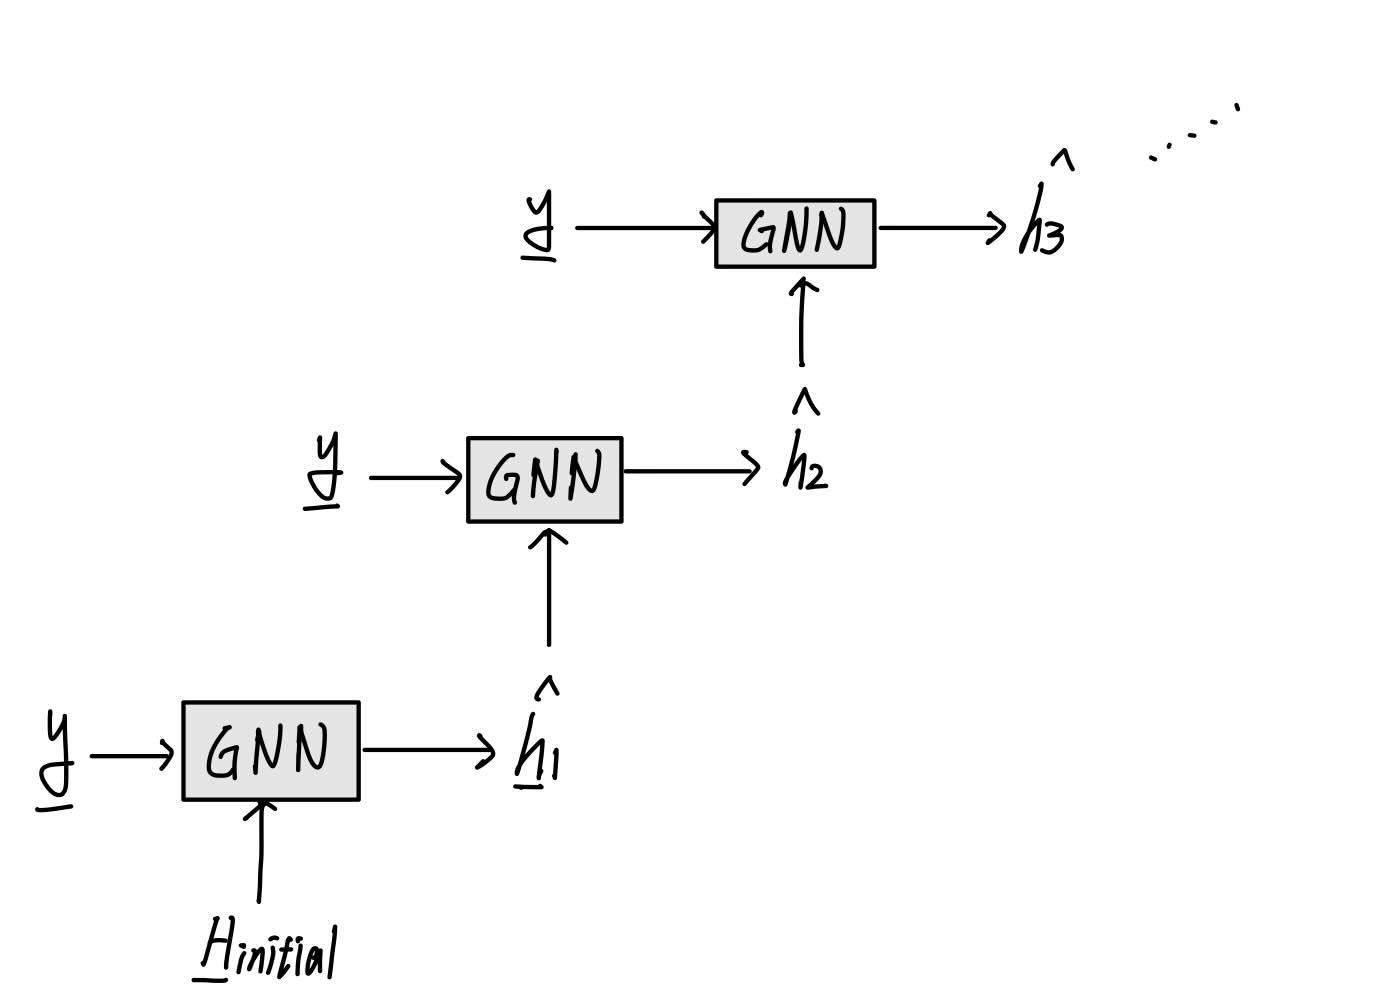
\includegraphics[width=.8\linewidth]{figures/Guess.jpg}\\
        I guess that using this method, the estimated $\hat{\H}$ will get increasingly better.

    \section{Simulation Result}

        %%%%%%%%%%%%% MLP structure

        % Simulation Configuration:\\
        \begin{table}[h] \label{tab:Configuration}
        \centering
        \renewcommand{\arraystretch}{1.5}
        \begin{tabular}{|c|c|}
            \hline
            parameters   &values \\
            \hline \hline
            [$n_R,n_T$,$T$]                 &[4,8,8]        \\ \hline
            $\mu_H, \sigma_H$               &0, 1          \\ \hline
            Hidden layer size               &1024 or 4$\times$1024   \\ \hline
            Length of each trajectory       &1                      \\ \hline
            Batch size = $|\mathcal{D}|$    &10,000         \\ \hline
            Number of batches               &100            \\ \hline
            Trainning dataset               &1,000,000      \\ \hline
            Validation dataset              &2,000          \\ \hline
            Epoch                           &200 $\sim$ 1,000   \\ \hline
            Learning rate                   &1e-5 $\sim$ 1e-6  \\ \hline
        \end{tabular}
        \caption{simulation configuration}
        \end{table}
        Let the loss be Normalized Mean Squared Error (NMSE):
        \begin{equation} \label{NMSE}
            NMSE=\frac{1}{N} \sum\limits_{n=1}^N
            \frac{\left\| \h_n-\phi(\mathbf{y}_n;\boldsymbol{\theta}_k) \right\|^2_2}
            {\left\| \h_n \right\|^2_2},
        \end{equation}
        where $N$ represents the size of the training or validation dataset, 
        implying that the Normalized Mean Squared Error (NMSE) is calculated for each epoch.\\
        %%%%%%%%%%%%%  Adam
        % Let step size $\alpha_{t,k}$ and $\alpha_{\lambda,k}$ to be ${\alpha_{t,0}}/{k}$
        % and ${\alpha_{\lambda,0}}/{k}$, where $k$ is the iteration index.

        % \begin{figure}[H]
        %     \centering
        %     \begin{subfigure}[b]{1\linewidth}
        %         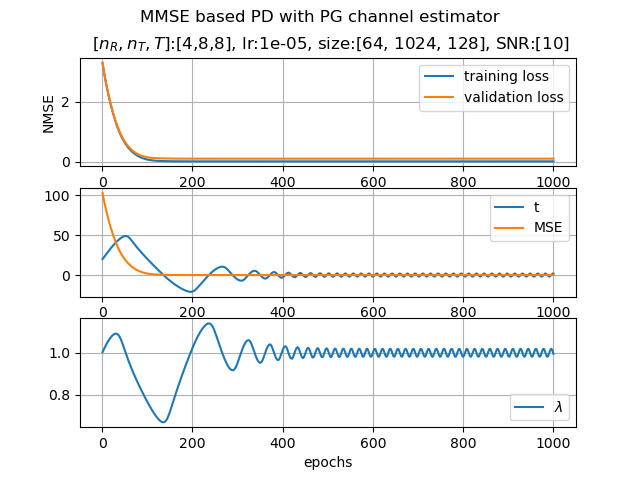
\includegraphics[width=\linewidth]{figures/lr1e-05_[64, 1024, 128]_ep1000_SNR_[10].png}
        %     %   \caption{lr: 1e-3, epoch: 100}
        %     %   \label{fig:image1}
        %     \end{subfigure}
        %     \begin{subfigure}[b]{1\linewidth}
        %         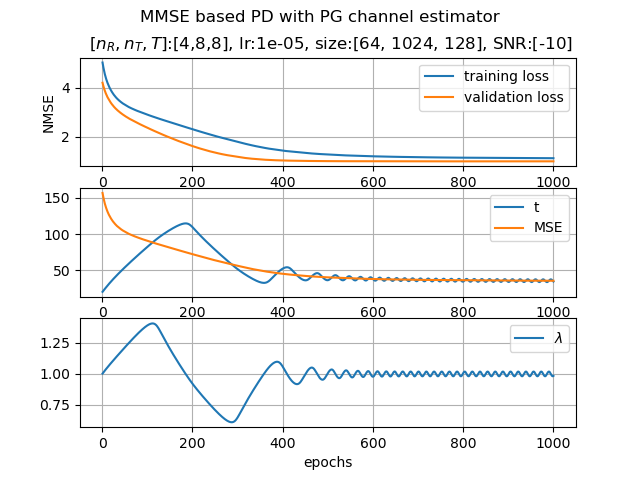
\includegraphics[width=\linewidth]{figures/lr1e-05_[64, 1024, 128]_ep1000_SNR_[-10].png}
        %     %   \caption{lr: 1e-3, epoch: 100}
        %     %   \label{fig:image2}
        %     \end{subfigure}
        %     \begin{subfigure}[b]{1\linewidth}
        %         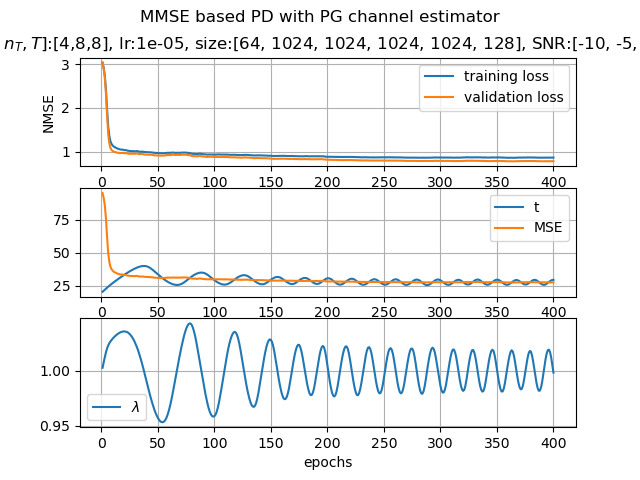
\includegraphics[width=\linewidth]{figures/lr1e-05_[64, 1024, 1024, 1024, 1024, 128]_ep400_SNR_[-10, -5, 5, 10].png}
        %     %   \caption{Image 3}
        %     %   \label{fig:image3}
        %     \end{subfigure}
        %     \caption{(a) 1 hidden layer MLP trained with SNR = 10
        %         (b) 1 hidden layer MLP trained with SNR = -10
        %         (c) 4 hidden layer MLP trained with SNR = -10, -5, 5, 10}
        %     \label{fig:train_result}
        % \end{figure}
        % \begin{figure}[h]
        %     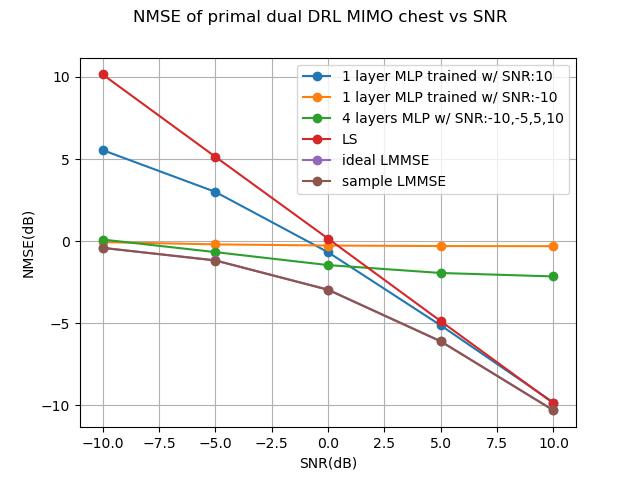
\includegraphics[width=\linewidth]{figures/3mlp_Chest_.png}
        %     \caption{performance of channel estimators under different SNRs}
        %     \label{fig:test_result}
        % \end{figure}

        \begin{figure}[h]
            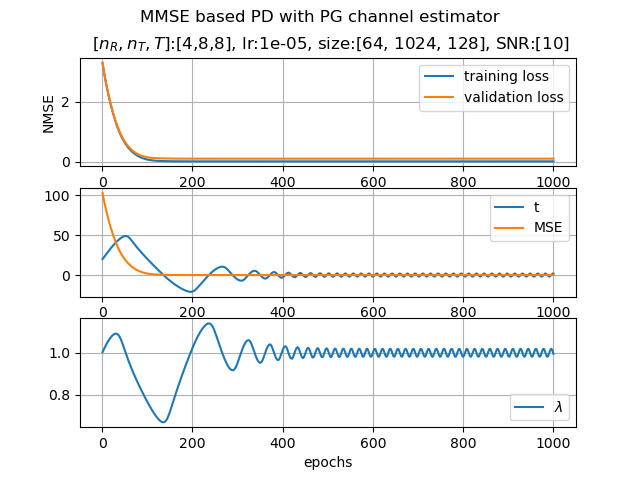
\includegraphics[width=\linewidth]{figures/lr1e-05_[64, 1024, 128]_ep1000_SNR_[10].png}
        %   \caption{lr: 1e-3, epoch: 100}
        %   \label{fig:image1}
        \end{figure}
        \begin{figure}[h]
            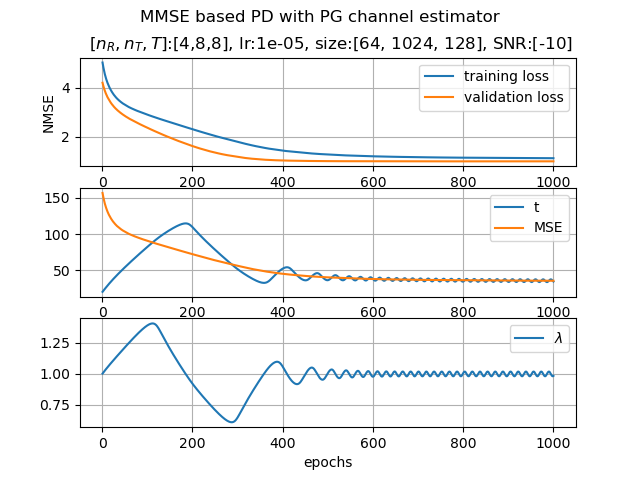
\includegraphics[width=\linewidth]{figures/lr1e-05_[64, 1024, 128]_ep1000_SNR_[-10].png}
        %   \caption{lr: 1e-3, epoch: 100}
        %   \label{fig:image2}
        \end{figure}
        \begin{figure}[h]
            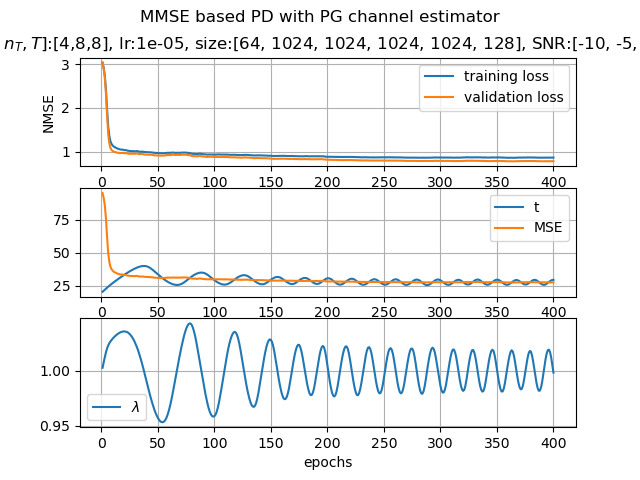
\includegraphics[width=\linewidth]{figures/lr1e-05_[64, 1024, 1024, 1024, 1024, 128]_ep400_SNR_[-10, -5, 5, 10].png}
        %   \caption{Image 3}
        %   \label{fig:image3}
            \caption{(a) 1 hidden layer MLP trained with SNR = 10
                (b) 1 hidden layer MLP trained with SNR = -10
                (c) 4 hidden layer MLP trained with SNR = -10, -5, 5, 10}
            \label{fig:train_result}
        \end{figure}
        \begin{figure}[h]
            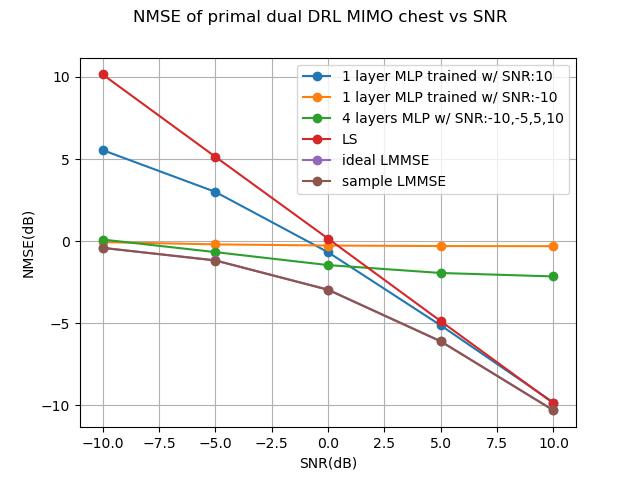
\includegraphics[width=\linewidth]{figures/3mlp_Chest_.png}
            \caption{performance of channel estimators under different SNRs}
            \label{fig:test_result}
        \end{figure}

        Figure (\ref{fig:train_result}) shows the training results of different sizes of MLPs trained with SNR values of \{10\}, \{-10\}, \{-10, -5, 5 10\}. 
        It displays the values of the primal and dual variables during the training process.

        Figure (\ref{fig:test_result}) shows the testing results of MLPs from Figure (\ref{fig:train_result}) under different SNRs, 
        compared with LS, sampled LMMSE, and ideal LMMSE estimators, where the ideal LMMSE is calculated using the ideal covariance matrix of $\H$: 
        $\C_{\h\h}(\C_{\h\h}+\C_{\w\w})^{-1}\y = \sigma_{\H}^2\I(\sigma_{\H}^2\I + \sigma_{\W}^2\I)^{-1}\y = \frac{\sigma_{\H}^2}{\sigma_{\H}^2+\sigma_{\W}^2}\y$
        and the sample LMMSE is calculated using $\H$ from testing dataset: $\C_{\h\h} = \frac{1}{N}\sum_{n=1}^{N}\h_n\h_n^T$, where $N$ is the size of testing dataset.

        % For MLP trained with SNR = 10, its NMSE is close to LMMSE when SNR is high, but perform bad when SNR is low; for MLP trained with SNR = -10, it's opposite.
        For the MLP trained with SNR = 10, its NMSE is close to that of the LMMSE when the SNR is high, but it performs poorly when the SNR is low. 
        Conversely, the MLP trained with SNR = -10 performs well at low SNRs but poorly at high SNRs.
        However, the MLP trained with 4 different SNRs performs well at low SNRs but poorly at high SNRs, similar to the second case.

    \section{Conclusion}
        In this work, we proposed a novel approach for MIMO channel estimation using a neural network-based minimum mean square error (MMSE) estimator, 
        trained via deep reinforcement learning (DRL) and a primal-dual optimization method. Our method leverages the power of neural networks to model 
        the complex relationship between the received signal and the channel state.

        The primal-dual optimization framework facilitates efficient training by iteratively updating the primal and dual variables using gradient descent and ascent. 
        The policy gradient method is employed to calculate the gradients, enabling the use of large neural network models without excessive computational costs.
        
        Our simulation results demonstrate that the proposed neural network-based MMSE estimator can outperform the least squares (LS) and approach the performance of 
        linear MMSE (LMMSE) estimators under specific signal-to-noise ratio (SNR) conditions, especially under challenging conditions with high noise levels. 
        However, it requires a larger model size to achieve robustness in its performance.
        
        Overall, the integration of DRL and primal-dual optimization with neural networks provides a powerful framework for tackling the MIMO channel estimation problem. 
        Future work may explore further enhancements, such as incorporating more sophisticated neural network architectures or extending the approach to 
        other types of communication channels and systems.









    % \bibliographystyle{abbrv}
    % \bibliography{mergedBib}
    % \vspace{1cm}

    \bibstyle{abbrv}
    \begin{thebibliography}{1}
    \bibitem{Carrson}
        C. C. Fung, and D. Ivakhnenkov, "Model-Driven Neural Network Based MIMO Channel Estimator".
    \bibitem{Eisen2019conf}
        M. Eisen and A. Ribeiro, ``Large scale wireless power allocation with graph neural networks,'' \emph{Proc. of the 2019 IEEE 20th Workshop on Signal Processing Advances in Wireless Communications (SPAWC)}, pp. 1-5, 2019.
    \bibitem{Eisen2019journal}
        M. Eisen, C. Zhang, L.F.O. Chamon, D.D. Lee and A. Ribeiro, ``Learning optimal power allocations in wireless systems,'' \emph{IEEE Trans. on Signal Processing}, vol. 67(10), pp. 2775-2790, May 2019.
    \bibitem{Eisen2020}
        M. Eisen and A. Ribeiro, ``Optimal wireless resource allocation with random edge graph neural networks,'' \emph{IEEE Trans. on Signal Processing}, vol. 68, pp. 2977-2991, 2020.
    \bibitem{Naderi2022}    
        N. NaderiAlizadeh, M. Eisen and A. Ribeiro, ``State-Augmented learnable algorithms for resource management in wireless networks,'' \emph{IEEE Trans. on Signal Processing}, vol. 70, pp. 5898-5912, Dec. 2022.
    \bibitem{Naderi2023}    
        N. NaderiAlizadeh, M. Eisen and A. Ribeiro, ``Learning resilient radio resource management policies with graph neural networks,'' \emph{IEEE Trans. on Signal Processing}, volo. 71, pp. 995-1009, Mar. 2023.
    % \bibitem{Naderi2024}
    %     S. Das, N. NaderiAlizadeh and A. Ribeiro, ``State-augmented information routing in communication systems with graph neural networks,''  \emph{IEEE Intl. Conf. on Acoustics, Speech and Signal Processing (ICASSP)}, Seoul, South Korea, Apr. 2024.
        % OpenAI Spinning Up introduction to RL Part 3: Intro to Policy Optimization %: \href{https://spinningup.openai.com/en/latest/spinningup/rl_intro3.html}
    \end{thebibliography}

\end{document}




